\documentclass[1p]{elsarticle_modified}
%\bibliographystyle{elsarticle-num}

%\usepackage[colorlinks]{hyperref}
%\usepackage{abbrmath_seonhwa} %\Abb, \Ascr, \Acal ,\Abf, \Afrak
\usepackage{amsfonts}
\usepackage{amssymb}
\usepackage{amsmath}
\usepackage{amsthm}
\usepackage{scalefnt}
\usepackage{amsbsy}
\usepackage{kotex}
\usepackage{caption}
\usepackage{subfig}
\usepackage{color}
\usepackage{graphicx}
\usepackage{xcolor} %% white, black, red, green, blue, cyan, magenta, yellow
\usepackage{float}
\usepackage{setspace}
\usepackage{hyperref}

\usepackage{tikz}
\usetikzlibrary{arrows}

\usepackage{multirow}
\usepackage{array} % fixed length table
\usepackage{hhline}

%%%%%%%%%%%%%%%%%%%%%
\makeatletter
\renewcommand*\env@matrix[1][\arraystretch]{%
	\edef\arraystretch{#1}%
	\hskip -\arraycolsep
	\let\@ifnextchar\new@ifnextchar
	\array{*\c@MaxMatrixCols c}}
\makeatother %https://tex.stackexchange.com/questions/14071/how-can-i-increase-the-line-spacing-in-a-matrix
%%%%%%%%%%%%%%%

\usepackage[normalem]{ulem}

\newcommand{\msout}[1]{\ifmmode\text{\sout{\ensuremath{#1}}}\else\sout{#1}\fi}
%SOURCE: \msout is \stkout macro in https://tex.stackexchange.com/questions/20609/strikeout-in-math-mode

\newcommand{\cancel}[1]{
	\ifmmode
	{\color{red}\msout{#1}}
	\else
	{\color{red}\sout{#1}}
	\fi
}

\newcommand{\add}[1]{
	{\color{blue}\uwave{#1}}
}

\newcommand{\replace}[2]{
	\ifmmode
	{\color{red}\msout{#1}}{\color{blue}\uwave{#2}}
	\else
	{\color{red}\sout{#1}}{\color{blue}\uwave{#2}}
	\fi
}

\newcommand{\Sol}{\mathcal{S}} %segment
\newcommand{\D}{D} %diagram
\newcommand{\A}{\mathcal{A}} %arc


%%%%%%%%%%%%%%%%%%%%%%%%%%%%%5 test

\def\sl{\operatorname{\textup{SL}}(2,\Cbb)}
\def\psl{\operatorname{\textup{PSL}}(2,\Cbb)}
\def\quan{\mkern 1mu \triangleright \mkern 1mu}

\theoremstyle{definition}
\newtheorem{thm}{Theorem}[section]
\newtheorem{prop}[thm]{Proposition}
\newtheorem{lem}[thm]{Lemma}
\newtheorem{ques}[thm]{Question}
\newtheorem{cor}[thm]{Corollary}
\newtheorem{defn}[thm]{Definition}
\newtheorem{exam}[thm]{Example}
\newtheorem{rmk}[thm]{Remark}
\newtheorem{alg}[thm]{Algorithm}

\newcommand{\I}{\sqrt{-1}}
\begin{document}

%\begin{frontmatter}
%
%\title{Boundary parabolic representations of knots up to 8 crossings}
%
%%% Group authors per affiliation:
%\author{Yunhi Cho} 
%\address{Department of Mathematics, University of Seoul, Seoul, Korea}
%\ead{yhcho@uos.ac.kr}
%
%
%\author{Seonhwa Kim} %\fnref{s_kim}}
%\address{Center for Geometry and Physics, Institute for Basic Science, Pohang, 37673, Korea}
%\ead{ryeona17@ibs.re.kr}
%
%\author{Hyuk Kim}
%\address{Department of Mathematical Sciences, Seoul National University, Seoul 08826, Korea}
%\ead{hyukkim@snu.ac.kr}
%
%\author{Seokbeom Yoon}
%\address{Department of Mathematical Sciences, Seoul National University, Seoul, 08826,  Korea}
%\ead{sbyoon15@snu.ac.kr}
%
%\begin{abstract}
%We find all boundary parabolic representation of knots up to 8 crossings.
%
%\end{abstract}
%\begin{keyword}
%    \MSC[2010] 57M25 
%\end{keyword}
%
%\end{frontmatter}

%\linenumbers
%\tableofcontents
%
\newcommand\colored[1]{\textcolor{white}{\rule[-0.35ex]{0.8em}{1.4ex}}\kern-0.8em\color{red} #1}%
%\newcommand\colored[1]{\textcolor{white}{ #1}\kern-2.17ex	\textcolor{white}{ #1}\kern-1.81ex	\textcolor{white}{ #1}\kern-2.15ex\color{red}#1	}

{\Large $\underline{12a_{0945}~(K12a_{0945})}$}

\setlength{\tabcolsep}{10pt}
\renewcommand{\arraystretch}{1.6}
\vspace{1cm}\begin{tabular}{m{100pt}>{\centering\arraybackslash}m{274pt}}
\multirow{5}{120pt}{
	\centering
	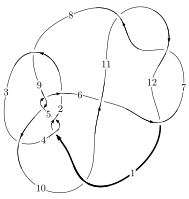
\includegraphics[width=112pt]{../../../GIT/diagram.site/Diagrams/png/1746_12a_0945.png}\\
\ \ \ A knot diagram\footnotemark}&
\allowdisplaybreaks
\textbf{Linearized knot diagam} \\
\cline{2-2}
 &
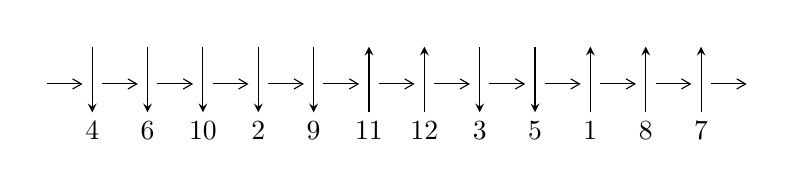
\begin{tikzpicture}[x=20pt, y=17pt]
	% nodes
	\node (C0) at (0, 0) {};
	\node (C1) at (1, 0) {};
	\node (C1U) at (1, +1) {};
	\node (C1D) at (1, -1) {4};

	\node (C2) at (2, 0) {};
	\node (C2U) at (2, +1) {};
	\node (C2D) at (2, -1) {6};

	\node (C3) at (3, 0) {};
	\node (C3U) at (3, +1) {};
	\node (C3D) at (3, -1) {10};

	\node (C4) at (4, 0) {};
	\node (C4U) at (4, +1) {};
	\node (C4D) at (4, -1) {2};

	\node (C5) at (5, 0) {};
	\node (C5U) at (5, +1) {};
	\node (C5D) at (5, -1) {9};

	\node (C6) at (6, 0) {};
	\node (C6U) at (6, +1) {};
	\node (C6D) at (6, -1) {11};

	\node (C7) at (7, 0) {};
	\node (C7U) at (7, +1) {};
	\node (C7D) at (7, -1) {12};

	\node (C8) at (8, 0) {};
	\node (C8U) at (8, +1) {};
	\node (C8D) at (8, -1) {3};

	\node (C9) at (9, 0) {};
	\node (C9U) at (9, +1) {};
	\node (C9D) at (9, -1) {5};

	\node (C10) at (10, 0) {};
	\node (C10U) at (10, +1) {};
	\node (C10D) at (10, -1) {1};

	\node (C11) at (11, 0) {};
	\node (C11U) at (11, +1) {};
	\node (C11D) at (11, -1) {8};

	\node (C12) at (12, 0) {};
	\node (C12U) at (12, +1) {};
	\node (C12D) at (12, -1) {7};
	\node (C13) at (13, 0) {};

	% arrows
	\draw[->,>={angle 60}]
	(C0) edge (C1) (C1) edge (C2) (C2) edge (C3) (C3) edge (C4) (C4) edge (C5) (C5) edge (C6) (C6) edge (C7) (C7) edge (C8) (C8) edge (C9) (C9) edge (C10) (C10) edge (C11) (C11) edge (C12) (C12) edge (C13) ;	\draw[->,>=stealth]
	(C1U) edge (C1D) (C2U) edge (C2D) (C3U) edge (C3D) (C4U) edge (C4D) (C5U) edge (C5D) (C6D) edge (C6U) (C7D) edge (C7U) (C8U) edge (C8D) (C9U) edge (C9D) (C10D) edge (C10U) (C11D) edge (C11U) (C12D) edge (C12U) ;
	\end{tikzpicture} \\
\hhline{~~} \\& 
\textbf{Solving Sequence} \\ \cline{2-2} 
 &
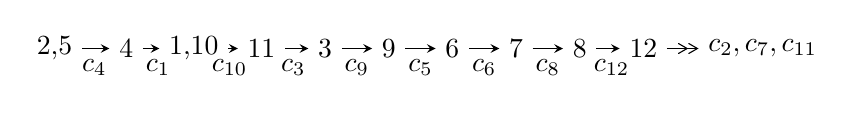
\begin{tikzpicture}[x=23pt, y=7pt]
	% node
	\node (A0) at (-1/8, 0) {2,5};
	\node (A1) at (1, 0) {4};
	\node (A2) at (33/16, 0) {1,10};
	\node (A3) at (25/8, 0) {11};
	\node (A4) at (33/8, 0) {3};
	\node (A5) at (41/8, 0) {9};
	\node (A6) at (49/8, 0) {6};
	\node (A7) at (57/8, 0) {7};
	\node (A8) at (65/8, 0) {8};
	\node (A9) at (73/8, 0) {12};
	\node (C1) at (1/2, -1) {$c_{4}$};
	\node (C2) at (3/2, -1) {$c_{1}$};
	\node (C3) at (21/8, -1) {$c_{10}$};
	\node (C4) at (29/8, -1) {$c_{3}$};
	\node (C5) at (37/8, -1) {$c_{9}$};
	\node (C6) at (45/8, -1) {$c_{5}$};
	\node (C7) at (53/8, -1) {$c_{6}$};
	\node (C8) at (61/8, -1) {$c_{8}$};
	\node (C9) at (69/8, -1) {$c_{12}$};
	\node (A10) at (11, 0) {$c_{2},c_{7},c_{11}$};

	% edge
	\draw[->,>=stealth]	
	(A0) edge (A1) (A1) edge (A2) (A2) edge (A3) (A3) edge (A4) (A4) edge (A5) (A5) edge (A6) (A6) edge (A7) (A7) edge (A8) (A8) edge (A9) ;
	\draw[->>,>={angle 60}]	
	(A9) edge (A10);
\end{tikzpicture} \\ 

\end{tabular} \\

\footnotetext{
The image of knot diagram is generated by the software ``\textbf{Draw programme}" developed by Andrew Bartholomew(\url{http://www.layer8.co.uk/maths/draw/index.htm\#Running-draw}), where we modified some parts for our purpose(\url{https://github.com/CATsTAILs/LinksPainter}).
}\phantom \\ \newline 
\centering \textbf{Ideals for irreducible components\footnotemark of $X_{\text{par}}$} 
 
\begin{align*}
I^u_{1}&=\langle 
1.02739\times10^{332} u^{98}-2.37382\times10^{331} u^{97}+\cdots+3.74964\times10^{331} b-1.45413\times10^{332},\\
\phantom{I^u_{1}}&\phantom{= \langle  }-1.49879\times10^{332} u^{98}+7.34438\times10^{331} u^{97}+\cdots+3.74964\times10^{331} a+3.88173\times10^{332},\\
\phantom{I^u_{1}}&\phantom{= \langle  }u^{99}- u^{98}+\cdots+23 u^2+1\rangle \\
\\
\end{align*}
\raggedright * 1 irreducible components of $\dim_{\mathbb{C}}=0$, with total 99 representations.\\
\footnotetext{All coefficients of polynomials are rational numbers. But the coefficients are sometimes approximated in decimal forms when there is not enough margin.}
\newpage
\renewcommand{\arraystretch}{1}
\centering \section*{I. $I^u_{1}= \langle 1.03\times10^{332} u^{98}-2.37\times10^{331} u^{97}+\cdots+3.75\times10^{331} b-1.45\times10^{332},\;-1.50\times10^{332} u^{98}+7.34\times10^{331} u^{97}+\cdots+3.75\times10^{331} a+3.88\times10^{332},\;u^{99}- u^{98}+\cdots+23 u^2+1 \rangle$}
\flushleft \textbf{(i) Arc colorings}\\
\begin{tabular}{m{7pt} m{180pt} m{7pt} m{180pt} }
\flushright $a_{2}=$&$\begin{pmatrix}0\\u\end{pmatrix}$ \\
\flushright $a_{5}=$&$\begin{pmatrix}1\\0\end{pmatrix}$ \\
\flushright $a_{4}=$&$\begin{pmatrix}1\\- u^2\end{pmatrix}$ \\
\flushright $a_{1}=$&$\begin{pmatrix}u\\- u^3+u\end{pmatrix}$ \\
\flushright $a_{10}=$&$\begin{pmatrix}3.99717 u^{98}-1.95869 u^{97}+\cdots+5.84289 u-10.3523\\-2.73998 u^{98}+0.633079 u^{97}+\cdots+11.1270 u+3.87805\end{pmatrix}$ \\
\flushright $a_{11}=$&$\begin{pmatrix}1.49086 u^{98}-1.37385 u^{97}+\cdots+10.6124 u-7.30046\\-3.56577 u^{98}+0.832592 u^{97}+\cdots+13.3902 u+5.00840\end{pmatrix}$ \\
\flushright $a_{3}=$&$\begin{pmatrix}1.93055 u^{98}-4.68758 u^{97}+\cdots+18.1992 u+7.78150\\0.155337 u^{98}-1.61346 u^{97}+\cdots-1.45150 u+2.25046\end{pmatrix}$ \\
\flushright $a_{9}=$&$\begin{pmatrix}1.25719 u^{98}-1.32561 u^{97}+\cdots+16.9699 u-6.47424\\-2.73998 u^{98}+0.633079 u^{97}+\cdots+11.1270 u+3.87805\end{pmatrix}$ \\
\flushright $a_{6}=$&$\begin{pmatrix}1.93654 u^{98}+1.72896 u^{97}+\cdots-27.0840 u-7.72022\\-4.92304 u^{98}+0.941981 u^{97}+\cdots+8.31108 u+5.39610\end{pmatrix}$ \\
\flushright $a_{7}=$&$\begin{pmatrix}0.371340 u^{98}+1.23713 u^{97}+\cdots-22.3156 u-0.337780\\1.37216 u^{98}-0.185051 u^{97}+\cdots-5.23013 u-2.09610\end{pmatrix}$ \\
\flushright $a_{8}=$&$\begin{pmatrix}0.277222 u^{98}-0.970149 u^{97}+\cdots+24.8608 u-5.43616\\-2.32353 u^{98}+0.371790 u^{97}+\cdots+10.4207 u+3.83701\end{pmatrix}$ \\
\flushright $a_{12}=$&$\begin{pmatrix}0.402554 u^{98}-0.156919 u^{97}+\cdots+23.0714 u-6.03950\\-1.47855 u^{98}+0.456172 u^{97}+\cdots+8.63301 u+1.93043\end{pmatrix}$\\&\end{tabular}
\flushleft \textbf{(ii) Obstruction class $= -1$}\\~\\
\flushleft \textbf{(iii) Cusp Shapes $= 4.12981 u^{98}+4.34684 u^{97}+\cdots-11.0775 u-8.25641$}\\~\\
\newpage\renewcommand{\arraystretch}{1}
\flushleft \textbf{(iv) u-Polynomials at the component}\newline \\
\begin{tabular}{m{50pt}|m{274pt}}
Crossings & \hspace{64pt}u-Polynomials at each crossing \\
\hline $$\begin{aligned}c_{1},c_{4}\end{aligned}$$&$\begin{aligned}
&u^{99}- u^{98}+\cdots+23 u^2+1
\end{aligned}$\\
\hline $$\begin{aligned}c_{2}\end{aligned}$$&$\begin{aligned}
&u^{99}-17 u^{98}+\cdots-188 u+19
\end{aligned}$\\
\hline $$\begin{aligned}c_{3}\end{aligned}$$&$\begin{aligned}
&u^{99}- u^{98}+\cdots+140544 u+38593
\end{aligned}$\\
\hline $$\begin{aligned}c_{5},c_{9}\end{aligned}$$&$\begin{aligned}
&u^{99}+3 u^{98}+\cdots+4 u+1
\end{aligned}$\\
\hline $$\begin{aligned}c_{6}\end{aligned}$$&$\begin{aligned}
&u^{99}+3 u^{98}+\cdots+27558 u+10961
\end{aligned}$\\
\hline $$\begin{aligned}c_{7},c_{11},c_{12}\end{aligned}$$&$\begin{aligned}
&u^{99}-3 u^{98}+\cdots-5 u^2+1
\end{aligned}$\\
\hline $$\begin{aligned}c_{8}\end{aligned}$$&$\begin{aligned}
&u^{99}+u^{98}+\cdots+2 u+1
\end{aligned}$\\
\hline $$\begin{aligned}c_{10}\end{aligned}$$&$\begin{aligned}
&u^{99}+17 u^{98}+\cdots-745808 u-47873
\end{aligned}$\\
\hline
\end{tabular}\\~\\
\newpage\renewcommand{\arraystretch}{1}
\flushleft \textbf{(v) Riley Polynomials at the component}\newline \\
\begin{tabular}{m{50pt}|m{274pt}}
Crossings & \hspace{64pt}Riley Polynomials at each crossing \\
\hline $$\begin{aligned}c_{1},c_{4}\end{aligned}$$&$\begin{aligned}
&y^{99}-65 y^{98}+\cdots-46 y-1
\end{aligned}$\\
\hline $$\begin{aligned}c_{2}\end{aligned}$$&$\begin{aligned}
&y^{99}+167 y^{98}+\cdots+15926 y-361
\end{aligned}$\\
\hline $$\begin{aligned}c_{3}\end{aligned}$$&$\begin{aligned}
&y^{99}-173 y^{98}+\cdots+31500556694 y-1489419649
\end{aligned}$\\
\hline $$\begin{aligned}c_{5},c_{9}\end{aligned}$$&$\begin{aligned}
&y^{99}+59 y^{98}+\cdots+10 y-1
\end{aligned}$\\
\hline $$\begin{aligned}c_{6}\end{aligned}$$&$\begin{aligned}
&y^{99}+23 y^{98}+\cdots-2411815078 y-120143521
\end{aligned}$\\
\hline $$\begin{aligned}c_{7},c_{11},c_{12}\end{aligned}$$&$\begin{aligned}
&y^{99}+91 y^{98}+\cdots+10 y-1
\end{aligned}$\\
\hline $$\begin{aligned}c_{8}\end{aligned}$$&$\begin{aligned}
&y^{99}+3 y^{98}+\cdots+66 y-1
\end{aligned}$\\
\hline $$\begin{aligned}c_{10}\end{aligned}$$&$\begin{aligned}
&y^{99}+63 y^{98}+\cdots+18472642594 y-2291824129
\end{aligned}$\\
\hline
\end{tabular}\\~\\
\newpage\flushleft \textbf{(vi) Complex Volumes and Cusp Shapes}
$$\begin{array}{c|c|c}  
\text{Solutions to }I^u_{1}& \I (\text{vol} + \sqrt{-1}CS) & \text{Cusp shape}\\
 \hline 
\begin{aligned}
u &= -0.994492 + 0.018996 I \\
a &= -8.09675 + 8.01488 I \\
b &= \phantom{-}0.036500 + 1.030300 I\end{aligned}
 & -5.85875 + 4.44226 I & \phantom{-0.000000 } 0 \\ \hline\begin{aligned}
u &= -0.994492 - 0.018996 I \\
a &= -8.09675 - 8.01488 I \\
b &= \phantom{-}0.036500 - 1.030300 I\end{aligned}
 & -5.85875 - 4.44226 I & \phantom{-0.000000 } 0 \\ \hline\begin{aligned}
u &= \phantom{-}0.975049 + 0.188085 I \\
a &= \phantom{-}1.70227 + 0.71514 I \\
b &= -0.86106 - 1.23598 I\end{aligned}
 & -0.83712 - 3.39889 I & \phantom{-0.000000 } 0 \\ \hline\begin{aligned}
u &= \phantom{-}0.975049 - 0.188085 I \\
a &= \phantom{-}1.70227 - 0.71514 I \\
b &= -0.86106 + 1.23598 I\end{aligned}
 & -0.83712 + 3.39889 I & \phantom{-0.000000 } 0 \\ \hline\begin{aligned}
u &= -0.983393 + 0.005334 I \\
a &= \phantom{-}10.61980 + 0.36470 I \\
b &= -0.046544 + 0.996080 I\end{aligned}
 & -0.29450 - 1.51441 I & \phantom{-0.000000 } 0 \\ \hline\begin{aligned}
u &= -0.983393 - 0.005334 I \\
a &= \phantom{-}10.61980 - 0.36470 I \\
b &= -0.046544 - 0.996080 I\end{aligned}
 & -0.29450 + 1.51441 I & \phantom{-0.000000 } 0 \\ \hline\begin{aligned}
u &= \phantom{-}0.940357 + 0.256776 I \\
a &= \phantom{-}1.52630 - 0.64498 I \\
b &= -1.120820 + 0.374656 I\end{aligned}
 & -3.47108 - 4.80291 I & \phantom{-0.000000 } 0 \\ \hline\begin{aligned}
u &= \phantom{-}0.940357 - 0.256776 I \\
a &= \phantom{-}1.52630 + 0.64498 I \\
b &= -1.120820 - 0.374656 I\end{aligned}
 & -3.47108 + 4.80291 I & \phantom{-0.000000 } 0 \\ \hline\begin{aligned}
u &= \phantom{-}1.015250 + 0.168887 I \\
a &= \phantom{-}0.501708 - 0.911504 I \\
b &= -0.40788 + 1.65089 I\end{aligned}
 & -5.64603 - 6.02681 I & \phantom{-0.000000 } 0 \\ \hline\begin{aligned}
u &= \phantom{-}1.015250 - 0.168887 I \\
a &= \phantom{-}0.501708 + 0.911504 I \\
b &= -0.40788 - 1.65089 I\end{aligned}
 & -5.64603 + 6.02681 I & \phantom{-0.000000 } 0\\
 \hline 
 \end{array}$$\newpage$$\begin{array}{c|c|c}  
\text{Solutions to }I^u_{1}& \I (\text{vol} + \sqrt{-1}CS) & \text{Cusp shape}\\
 \hline 
\begin{aligned}
u &= \phantom{-}0.372488 + 0.867010 I \\
a &= \phantom{-}0.0622155 - 0.1044290 I \\
b &= \phantom{-}0.329059 - 1.244270 I\end{aligned}
 & \phantom{-}5.94439 + 2.18444 I & \phantom{-0.000000 } 0 \\ \hline\begin{aligned}
u &= \phantom{-}0.372488 - 0.867010 I \\
a &= \phantom{-}0.0622155 + 0.1044290 I \\
b &= \phantom{-}0.329059 + 1.244270 I\end{aligned}
 & \phantom{-}5.94439 - 2.18444 I & \phantom{-0.000000 } 0 \\ \hline\begin{aligned}
u &= \phantom{-}0.305094 + 1.030890 I \\
a &= \phantom{-}0.056979 + 0.202482 I \\
b &= -0.357545 + 1.219710 I\end{aligned}
 & \phantom{-}2.48048 + 5.30165 I & \phantom{-0.000000 } 0 \\ \hline\begin{aligned}
u &= \phantom{-}0.305094 - 1.030890 I \\
a &= \phantom{-}0.056979 - 0.202482 I \\
b &= -0.357545 - 1.219710 I\end{aligned}
 & \phantom{-}2.48048 - 5.30165 I & \phantom{-0.000000 } 0 \\ \hline\begin{aligned}
u &= \phantom{-}0.901677 + 0.097789 I \\
a &= -0.216939 + 1.082560 I \\
b &= \phantom{-}0.20471 - 1.71903 I\end{aligned}
 & \phantom{-}0.62004 - 2.35166 I & \phantom{-0.000000 } 0 \\ \hline\begin{aligned}
u &= \phantom{-}0.901677 - 0.097789 I \\
a &= -0.216939 - 1.082560 I \\
b &= \phantom{-}0.20471 + 1.71903 I\end{aligned}
 & \phantom{-}0.62004 + 2.35166 I & \phantom{-0.000000 } 0 \\ \hline\begin{aligned}
u &= -0.509715 + 0.746888 I \\
a &= -0.169108 + 0.504425 I \\
b &= \phantom{-}0.533589 + 0.088687 I\end{aligned}
 & -7.28561 - 1.78675 I & \phantom{-0.000000 } 0 \\ \hline\begin{aligned}
u &= -0.509715 - 0.746888 I \\
a &= -0.169108 - 0.504425 I \\
b &= \phantom{-}0.533589 - 0.088687 I\end{aligned}
 & -7.28561 + 1.78675 I & \phantom{-0.000000 } 0 \\ \hline\begin{aligned}
u &= -0.222287 + 0.862791 I \\
a &= \phantom{-}0.302618 - 0.658490 I \\
b &= -0.607223 - 0.026295 I\end{aligned}
 & -6.34251 + 7.39460 I & \phantom{-0.000000 } 0 \\ \hline\begin{aligned}
u &= -0.222287 - 0.862791 I \\
a &= \phantom{-}0.302618 + 0.658490 I \\
b &= -0.607223 + 0.026295 I\end{aligned}
 & -6.34251 - 7.39460 I & \phantom{-0.000000 } 0\\
 \hline 
 \end{array}$$\newpage$$\begin{array}{c|c|c}  
\text{Solutions to }I^u_{1}& \I (\text{vol} + \sqrt{-1}CS) & \text{Cusp shape}\\
 \hline 
\begin{aligned}
u &= \phantom{-}1.025930 + 0.444337 I \\
a &= \phantom{-}1.71502 + 0.33410 I \\
b &= -0.661676 - 1.231940 I\end{aligned}
 & \phantom{-}0.29849 - 3.48845 I & \phantom{-0.000000 } 0 \\ \hline\begin{aligned}
u &= \phantom{-}1.025930 - 0.444337 I \\
a &= \phantom{-}1.71502 - 0.33410 I \\
b &= -0.661676 + 1.231940 I\end{aligned}
 & \phantom{-}0.29849 + 3.48845 I & \phantom{-0.000000 } 0 \\ \hline\begin{aligned}
u &= -1.105620 + 0.182833 I \\
a &= -1.53301 + 0.66453 I \\
b &= \phantom{-}0.149783 - 0.858878 I\end{aligned}
 & -0.893637 + 0.928581 I & \phantom{-0.000000 } 0 \\ \hline\begin{aligned}
u &= -1.105620 - 0.182833 I \\
a &= -1.53301 - 0.66453 I \\
b &= \phantom{-}0.149783 + 0.858878 I\end{aligned}
 & -0.893637 - 0.928581 I & \phantom{-0.000000 } 0 \\ \hline\begin{aligned}
u &= -1.052710 + 0.386949 I \\
a &= -0.139428 + 0.138796 I \\
b &= \phantom{-}0.348717 + 0.244272 I\end{aligned}
 & -4.88550 + 1.29779 I & \phantom{-0.000000 } 0 \\ \hline\begin{aligned}
u &= -1.052710 - 0.386949 I \\
a &= -0.139428 - 0.138796 I \\
b &= \phantom{-}0.348717 - 0.244272 I\end{aligned}
 & -4.88550 - 1.29779 I & \phantom{-0.000000 } 0 \\ \hline\begin{aligned}
u &= \phantom{-}0.490947 + 0.724635 I \\
a &= -0.115757 - 0.091258 I \\
b &= -0.308124 + 1.285350 I\end{aligned}
 & \phantom{-}1.98588 - 0.94910 I & \phantom{-0.000000 } 0 \\ \hline\begin{aligned}
u &= \phantom{-}0.490947 - 0.724635 I \\
a &= -0.115757 + 0.091258 I \\
b &= -0.308124 - 1.285350 I\end{aligned}
 & \phantom{-}1.98588 + 0.94910 I & \phantom{-0.000000 } 0 \\ \hline\begin{aligned}
u &= \phantom{-}0.024409 + 1.144880 I \\
a &= \phantom{-}0.161084 + 0.384659 I \\
b &= -0.368663 + 1.164000 I\end{aligned}
 & \phantom{-}1.78944 + 4.02340 I & \phantom{-0.000000 } 0 \\ \hline\begin{aligned}
u &= \phantom{-}0.024409 - 1.144880 I \\
a &= \phantom{-}0.161084 - 0.384659 I \\
b &= -0.368663 - 1.164000 I\end{aligned}
 & \phantom{-}1.78944 - 4.02340 I & \phantom{-0.000000 } 0\\
 \hline 
 \end{array}$$\newpage$$\begin{array}{c|c|c}  
\text{Solutions to }I^u_{1}& \I (\text{vol} + \sqrt{-1}CS) & \text{Cusp shape}\\
 \hline 
\begin{aligned}
u &= -0.725573 + 0.425618 I \\
a &= \phantom{-}1.29629 + 1.12020 I \\
b &= -0.236866 + 0.999057 I\end{aligned}
 & \phantom{-}1.10389 + 2.20019 I & \phantom{-0.000000 } 0 \\ \hline\begin{aligned}
u &= -0.725573 - 0.425618 I \\
a &= \phantom{-}1.29629 - 1.12020 I \\
b &= -0.236866 - 0.999057 I\end{aligned}
 & \phantom{-}1.10389 - 2.20019 I & \phantom{-0.000000 } 0 \\ \hline\begin{aligned}
u &= -0.844241 + 0.798032 I \\
a &= -0.781444 - 0.619640 I \\
b &= \phantom{-}0.326365 - 0.989143 I\end{aligned}
 & -3.03348 + 4.34292 I & \phantom{-0.000000 } 0 \\ \hline\begin{aligned}
u &= -0.844241 - 0.798032 I \\
a &= -0.781444 + 0.619640 I \\
b &= \phantom{-}0.326365 + 0.989143 I\end{aligned}
 & -3.03348 - 4.34292 I & \phantom{-0.000000 } 0 \\ \hline\begin{aligned}
u &= -0.814307 + 0.082370 I \\
a &= -3.09073 - 1.58258 I \\
b &= \phantom{-}0.147889 - 1.005710 I\end{aligned}
 & -1.93903 + 0.16998 I & \phantom{-0.000000 } 0 \\ \hline\begin{aligned}
u &= -0.814307 - 0.082370 I \\
a &= -3.09073 + 1.58258 I \\
b &= \phantom{-}0.147889 + 1.005710 I\end{aligned}
 & -1.93903 - 0.16998 I & \phantom{-0.000000 } 0 \\ \hline\begin{aligned}
u &= \phantom{-}0.818015 + 0.013466 I \\
a &= -1.83249 + 0.88185 I \\
b &= \phantom{-}1.032470 - 0.802275 I\end{aligned}
 & \phantom{-}1.061010 - 0.905393 I & \phantom{-0.000000 } 0 \\ \hline\begin{aligned}
u &= \phantom{-}0.818015 - 0.013466 I \\
a &= -1.83249 - 0.88185 I \\
b &= \phantom{-}1.032470 + 0.802275 I\end{aligned}
 & \phantom{-}1.061010 + 0.905393 I & \phantom{-0.000000 } 0 \\ \hline\begin{aligned}
u &= \phantom{-}1.171430 + 0.160474 I \\
a &= -1.35590 - 0.61144 I \\
b &= \phantom{-}0.73024 + 1.40259 I\end{aligned}
 & -8.18419 - 5.25528 I & \phantom{-0.000000 } 0 \\ \hline\begin{aligned}
u &= \phantom{-}1.171430 - 0.160474 I \\
a &= -1.35590 + 0.61144 I \\
b &= \phantom{-}0.73024 - 1.40259 I\end{aligned}
 & -8.18419 + 5.25528 I & \phantom{-0.000000 } 0\\
 \hline 
 \end{array}$$\newpage$$\begin{array}{c|c|c}  
\text{Solutions to }I^u_{1}& \I (\text{vol} + \sqrt{-1}CS) & \text{Cusp shape}\\
 \hline 
\begin{aligned}
u &= -0.814684\phantom{ +0.000000I} \\
a &= -0.0793313\phantom{ +0.000000I} \\
b &= -0.268977\phantom{ +0.000000I}\end{aligned}
 & -1.15052\phantom{ +0.000000I} & -10.1560\phantom{ +0.000000I} \\ \hline\begin{aligned}
u &= -0.201959 + 0.761271 I \\
a &= -0.248856 + 0.715476 I \\
b &= \phantom{-}0.583104 + 0.002888 I\end{aligned}
 & -0.70303 + 4.11723 I & \phantom{-0.000000 } 0 \\ \hline\begin{aligned}
u &= -0.201959 - 0.761271 I \\
a &= -0.248856 - 0.715476 I \\
b &= \phantom{-}0.583104 - 0.002888 I\end{aligned}
 & -0.70303 - 4.11723 I & \phantom{-0.000000 } 0 \\ \hline\begin{aligned}
u &= -0.133156 + 1.210760 I \\
a &= -0.248294 - 0.438800 I \\
b &= \phantom{-}0.378986 - 1.135900 I\end{aligned}
 & -4.35827 + 1.78343 I & \phantom{-0.000000 } 0 \\ \hline\begin{aligned}
u &= -0.133156 - 1.210760 I \\
a &= -0.248294 + 0.438800 I \\
b &= \phantom{-}0.378986 + 1.135900 I\end{aligned}
 & -4.35827 - 1.78343 I & \phantom{-0.000000 } 0 \\ \hline\begin{aligned}
u &= \phantom{-}1.113910 + 0.518276 I \\
a &= -1.63257 - 0.22728 I \\
b &= \phantom{-}0.627590 + 1.260540 I\end{aligned}
 & \phantom{-}3.60786 - 7.23643 I & \phantom{-0.000000 } 0 \\ \hline\begin{aligned}
u &= \phantom{-}1.113910 - 0.518276 I \\
a &= -1.63257 + 0.22728 I \\
b &= \phantom{-}0.627590 - 1.260540 I\end{aligned}
 & \phantom{-}3.60786 + 7.23643 I & \phantom{-0.000000 } 0 \\ \hline\begin{aligned}
u &= \phantom{-}0.091381 + 1.259280 I \\
a &= -0.206832 - 0.324273 I \\
b &= \phantom{-}0.389645 - 1.173270 I\end{aligned}
 & \phantom{-}2.61420 + 7.82431 I & \phantom{-0.000000 } 0 \\ \hline\begin{aligned}
u &= \phantom{-}0.091381 - 1.259280 I \\
a &= -0.206832 + 0.324273 I \\
b &= \phantom{-}0.389645 + 1.173270 I\end{aligned}
 & \phantom{-}2.61420 - 7.82431 I & \phantom{-0.000000 } 0 \\ \hline\begin{aligned}
u &= \phantom{-}1.270440 + 0.319765 I \\
a &= \phantom{-}1.323150 - 0.301719 I \\
b &= -1.147510 + 0.129638 I\end{aligned}
 & -6.03634 - 3.86723 I & \phantom{-0.000000 } 0\\
 \hline 
 \end{array}$$\newpage$$\begin{array}{c|c|c}  
\text{Solutions to }I^u_{1}& \I (\text{vol} + \sqrt{-1}CS) & \text{Cusp shape}\\
 \hline 
\begin{aligned}
u &= \phantom{-}1.270440 - 0.319765 I \\
a &= \phantom{-}1.323150 + 0.301719 I \\
b &= -1.147510 - 0.129638 I\end{aligned}
 & -6.03634 + 3.86723 I & \phantom{-0.000000 } 0 \\ \hline\begin{aligned}
u &= \phantom{-}1.186390 + 0.567593 I \\
a &= \phantom{-}1.57142 + 0.16120 I \\
b &= -0.60806 - 1.27771 I\end{aligned}
 & -0.32932 - 10.94210 I & \phantom{-0.000000 } 0 \\ \hline\begin{aligned}
u &= \phantom{-}1.186390 - 0.567593 I \\
a &= \phantom{-}1.57142 - 0.16120 I \\
b &= -0.60806 + 1.27771 I\end{aligned}
 & -0.32932 + 10.94210 I & \phantom{-0.000000 } 0 \\ \hline\begin{aligned}
u &= -0.351502 + 0.583602 I \\
a &= \phantom{-}0.045268 - 0.641591 I \\
b &= -0.505707 - 0.020078 I\end{aligned}
 & -1.42824 + 0.58824 I & -6.32763 + 0. I\phantom{ +0.000000I} \\ \hline\begin{aligned}
u &= -0.351502 - 0.583602 I \\
a &= \phantom{-}0.045268 + 0.641591 I \\
b &= -0.505707 + 0.020078 I\end{aligned}
 & -1.42824 - 0.58824 I & -6.32763 + 0. I\phantom{ +0.000000I} \\ \hline\begin{aligned}
u &= \phantom{-}0.080166 + 1.328970 I \\
a &= \phantom{-}0.239652 + 0.318158 I \\
b &= -0.400675 + 1.169980 I\end{aligned}
 & -3.08712 + 11.21620 I & \phantom{-0.000000 } 0 \\ \hline\begin{aligned}
u &= \phantom{-}0.080166 - 1.328970 I \\
a &= \phantom{-}0.239652 - 0.318158 I \\
b &= -0.400675 - 1.169980 I\end{aligned}
 & -3.08712 - 11.21620 I & \phantom{-0.000000 } 0 \\ \hline\begin{aligned}
u &= \phantom{-}1.293750 + 0.385495 I \\
a &= -1.268880 + 0.317852 I \\
b &= \phantom{-}1.120670 - 0.123023 I\end{aligned}
 & -5.16454 - 8.24227 I & \phantom{-0.000000 } 0 \\ \hline\begin{aligned}
u &= \phantom{-}1.293750 - 0.385495 I \\
a &= -1.268880 - 0.317852 I \\
b &= \phantom{-}1.120670 + 0.123023 I\end{aligned}
 & -5.16454 + 8.24227 I & \phantom{-0.000000 } 0 \\ \hline\begin{aligned}
u &= \phantom{-}1.335970 + 0.253610 I \\
a &= -1.323960 + 0.222139 I \\
b &= \phantom{-}1.164640 - 0.095026 I\end{aligned}
 & -12.94020 - 1.45742 I & \phantom{-0.000000 } 0\\
 \hline 
 \end{array}$$\newpage$$\begin{array}{c|c|c}  
\text{Solutions to }I^u_{1}& \I (\text{vol} + \sqrt{-1}CS) & \text{Cusp shape}\\
 \hline 
\begin{aligned}
u &= \phantom{-}1.335970 - 0.253610 I \\
a &= -1.323960 - 0.222139 I \\
b &= \phantom{-}1.164640 + 0.095026 I\end{aligned}
 & -12.94020 + 1.45742 I & \phantom{-0.000000 } 0 \\ \hline\begin{aligned}
u &= \phantom{-}1.332610 + 0.410531 I \\
a &= \phantom{-}1.238100 - 0.304781 I \\
b &= -1.111890 + 0.110138 I\end{aligned}
 & -11.0505 - 11.9189 I & \phantom{-0.000000 } 0 \\ \hline\begin{aligned}
u &= \phantom{-}1.332610 - 0.410531 I \\
a &= \phantom{-}1.238100 + 0.304781 I \\
b &= -1.111890 - 0.110138 I\end{aligned}
 & -11.0505 + 11.9189 I & \phantom{-0.000000 } 0 \\ \hline\begin{aligned}
u &= -1.42681 + 0.24216 I \\
a &= \phantom{-}0.712034 - 0.124915 I \\
b &= -0.285167 + 0.736373 I\end{aligned}
 & -5.40693 + 1.49418 I & \phantom{-0.000000 } 0 \\ \hline\begin{aligned}
u &= -1.42681 - 0.24216 I \\
a &= \phantom{-}0.712034 + 0.124915 I \\
b &= -0.285167 - 0.736373 I\end{aligned}
 & -5.40693 - 1.49418 I & \phantom{-0.000000 } 0 \\ \hline\begin{aligned}
u &= \phantom{-}1.34786 + 0.55727 I \\
a &= \phantom{-}1.43150 + 0.12722 I \\
b &= -0.59525 - 1.31276 I\end{aligned}
 & -2.33740 - 9.95857 I & \phantom{-0.000000 } 0 \\ \hline\begin{aligned}
u &= \phantom{-}1.34786 - 0.55727 I \\
a &= \phantom{-}1.43150 - 0.12722 I \\
b &= -0.59525 + 1.31276 I\end{aligned}
 & -2.33740 + 9.95857 I & \phantom{-0.000000 } 0 \\ \hline\begin{aligned}
u &= \phantom{-}1.38738 + 0.50905 I \\
a &= -1.386450 - 0.150028 I \\
b &= \phantom{-}0.59836 + 1.32454 I\end{aligned}
 & -9.12270 - 7.60585 I & \phantom{-0.000000 } 0 \\ \hline\begin{aligned}
u &= \phantom{-}1.38738 - 0.50905 I \\
a &= -1.386450 + 0.150028 I \\
b &= \phantom{-}0.59836 - 1.32454 I\end{aligned}
 & -9.12270 + 7.60585 I & \phantom{-0.000000 } 0 \\ \hline\begin{aligned}
u &= -1.45704 + 0.27018 I \\
a &= \phantom{-}0.329760 - 0.023893 I \\
b &= -0.353412 - 0.464496 I\end{aligned}
 & -3.73507 + 1.99100 I & \phantom{-0.000000 } 0\\
 \hline 
 \end{array}$$\newpage$$\begin{array}{c|c|c}  
\text{Solutions to }I^u_{1}& \I (\text{vol} + \sqrt{-1}CS) & \text{Cusp shape}\\
 \hline 
\begin{aligned}
u &= -1.45704 - 0.27018 I \\
a &= \phantom{-}0.329760 + 0.023893 I \\
b &= -0.353412 + 0.464496 I\end{aligned}
 & -3.73507 - 1.99100 I & \phantom{-0.000000 } 0 \\ \hline\begin{aligned}
u &= \phantom{-}1.36786 + 0.59962 I \\
a &= -1.42831 - 0.09018 I \\
b &= \phantom{-}0.58643 + 1.31207 I\end{aligned}
 & -1.4502 - 14.2394 I & \phantom{-0.000000 } 0 \\ \hline\begin{aligned}
u &= \phantom{-}1.36786 - 0.59962 I \\
a &= -1.42831 + 0.09018 I \\
b &= \phantom{-}0.58643 - 1.31207 I\end{aligned}
 & -1.4502 + 14.2394 I & \phantom{-0.000000 } 0 \\ \hline\begin{aligned}
u &= \phantom{-}0.137003 + 0.479807 I \\
a &= \phantom{-}0.415392 - 1.273760 I \\
b &= -0.573266 + 0.183599 I\end{aligned}
 & -1.49366 + 1.81906 I & -1.74281 - 3.69548 I \\ \hline\begin{aligned}
u &= \phantom{-}0.137003 - 0.479807 I \\
a &= \phantom{-}0.415392 + 1.273760 I \\
b &= -0.573266 - 0.183599 I\end{aligned}
 & -1.49366 - 1.81906 I & -1.74281 + 3.69548 I \\ \hline\begin{aligned}
u &= -1.33451 + 0.72094 I \\
a &= -0.795110 - 0.245516 I \\
b &= \phantom{-}0.365795 - 0.879457 I\end{aligned}
 & -2.92305 + 1.66150 I & \phantom{-0.000000 } 0 \\ \hline\begin{aligned}
u &= -1.33451 - 0.72094 I \\
a &= -0.795110 + 0.245516 I \\
b &= \phantom{-}0.365795 + 0.879457 I\end{aligned}
 & -2.92305 - 1.66150 I & \phantom{-0.000000 } 0 \\ \hline\begin{aligned}
u &= -1.51217 + 0.15103 I \\
a &= -0.384725 - 0.022882 I \\
b &= \phantom{-}0.336258 + 0.528779 I\end{aligned}
 & -3.83043 - 1.65845 I & \phantom{-0.000000 } 0 \\ \hline\begin{aligned}
u &= -1.51217 - 0.15103 I \\
a &= -0.384725 + 0.022882 I \\
b &= \phantom{-}0.336258 - 0.528779 I\end{aligned}
 & -3.83043 + 1.65845 I & \phantom{-0.000000 } 0 \\ \hline\begin{aligned}
u &= \phantom{-}1.39495 + 0.61409 I \\
a &= \phantom{-}1.41261 + 0.07302 I \\
b &= -0.58199 - 1.31505 I\end{aligned}
 & -7.2935 - 17.8795 I & \phantom{-0.000000 } 0\\
 \hline 
 \end{array}$$\newpage$$\begin{array}{c|c|c}  
\text{Solutions to }I^u_{1}& \I (\text{vol} + \sqrt{-1}CS) & \text{Cusp shape}\\
 \hline 
\begin{aligned}
u &= \phantom{-}1.39495 - 0.61409 I \\
a &= \phantom{-}1.41261 - 0.07302 I \\
b &= -0.58199 + 1.31505 I\end{aligned}
 & -7.2935 + 17.8795 I & \phantom{-0.000000 } 0 \\ \hline\begin{aligned}
u &= -1.28110 + 0.84155 I \\
a &= \phantom{-}0.760307 + 0.307367 I \\
b &= -0.379856 + 0.907214 I\end{aligned}
 & -2.60113 + 5.38027 I & \phantom{-0.000000 } 0 \\ \hline\begin{aligned}
u &= -1.28110 - 0.84155 I \\
a &= \phantom{-}0.760307 - 0.307367 I \\
b &= -0.379856 - 0.907214 I\end{aligned}
 & -2.60113 - 5.38027 I & \phantom{-0.000000 } 0 \\ \hline\begin{aligned}
u &= -1.51624 + 0.33515 I \\
a &= -0.348799 + 0.058863 I \\
b &= \phantom{-}0.393435 + 0.465014 I\end{aligned}
 & -9.58932 + 4.99478 I & \phantom{-0.000000 } 0 \\ \hline\begin{aligned}
u &= -1.51624 - 0.33515 I \\
a &= -0.348799 - 0.058863 I \\
b &= \phantom{-}0.393435 - 0.465014 I\end{aligned}
 & -9.58932 - 4.99478 I & \phantom{-0.000000 } 0 \\ \hline\begin{aligned}
u &= -1.32704 + 0.90872 I \\
a &= -0.723788 - 0.302511 I \\
b &= \phantom{-}0.397500 - 0.908490 I\end{aligned}
 & -8.44003 + 8.52317 I & \phantom{-0.000000 } 0 \\ \hline\begin{aligned}
u &= -1.32704 - 0.90872 I \\
a &= -0.723788 + 0.302511 I \\
b &= \phantom{-}0.397500 + 0.908490 I\end{aligned}
 & -8.44003 - 8.52317 I & \phantom{-0.000000 } 0 \\ \hline\begin{aligned}
u &= -1.60381 + 0.15830 I \\
a &= \phantom{-}0.418149 - 0.011118 I \\
b &= -0.375095 - 0.547160 I\end{aligned}
 & -9.73725 - 4.53902 I & \phantom{-0.000000 } 0 \\ \hline\begin{aligned}
u &= -1.60381 - 0.15830 I \\
a &= \phantom{-}0.418149 + 0.011118 I \\
b &= -0.375095 + 0.547160 I\end{aligned}
 & -9.73725 + 4.53902 I & \phantom{-0.000000 } 0 \\ \hline\begin{aligned}
u &= -1.44341 + 0.73730 I \\
a &= \phantom{-}0.746384 + 0.216819 I \\
b &= -0.387157 + 0.863065 I\end{aligned}
 & -8.91446 - 1.06218 I & \phantom{-0.000000 } 0\\
 \hline 
 \end{array}$$\newpage$$\begin{array}{c|c|c}  
\text{Solutions to }I^u_{1}& \I (\text{vol} + \sqrt{-1}CS) & \text{Cusp shape}\\
 \hline 
\begin{aligned}
u &= -1.44341 - 0.73730 I \\
a &= \phantom{-}0.746384 - 0.216819 I \\
b &= -0.387157 - 0.863065 I\end{aligned}
 & -8.91446 + 1.06218 I & \phantom{-0.000000 } 0 \\ \hline\begin{aligned}
u &= \phantom{-}0.263548 + 0.166515 I \\
a &= \phantom{-}3.54408 + 1.76475 I \\
b &= -0.391506 - 0.811020 I\end{aligned}
 & -3.86603 + 4.15313 I & -1.33182 - 1.44818 I \\ \hline\begin{aligned}
u &= \phantom{-}0.263548 - 0.166515 I \\
a &= \phantom{-}3.54408 - 1.76475 I \\
b &= -0.391506 + 0.811020 I\end{aligned}
 & -3.86603 - 4.15313 I & -1.33182 + 1.44818 I \\ \hline\begin{aligned}
u &= \phantom{-}0.291799 + 0.090574 I \\
a &= -1.56516 + 2.32607 I \\
b &= \phantom{-}0.466028 - 0.523896 I\end{aligned}
 & \phantom{-}1.26906 - 0.95925 I & \phantom{-}4.32293 + 1.61283 I \\ \hline\begin{aligned}
u &= \phantom{-}0.291799 - 0.090574 I \\
a &= -1.56516 - 2.32607 I \\
b &= \phantom{-}0.466028 + 0.523896 I\end{aligned}
 & \phantom{-}1.26906 + 0.95925 I & \phantom{-}4.32293 - 1.61283 I \\ \hline\begin{aligned}
u &= -0.168662 + 0.052708 I \\
a &= -3.79045 + 6.49188 I \\
b &= \phantom{-}0.166465 + 1.024460 I\end{aligned}
 & -4.37987 - 4.27329 I & -3.90810 + 4.27086 I \\ \hline\begin{aligned}
u &= -0.168662 - 0.052708 I \\
a &= -3.79045 - 6.49188 I \\
b &= \phantom{-}0.166465 - 1.024460 I\end{aligned}
 & -4.37987 + 4.27329 I & -3.90810 - 4.27086 I \\ \hline\begin{aligned}
u &= -0.0185879 + 0.1145680 I \\
a &= -6.90872 + 3.17394 I \\
b &= -0.106809 + 1.097290 I\end{aligned}
 & \phantom{-}1.24428 + 1.65585 I & \phantom{-}0.29239 - 4.10547 I \\ \hline\begin{aligned}
u &= -0.0185879 - 0.1145680 I \\
a &= -6.90872 - 3.17394 I \\
b &= -0.106809 - 1.097290 I\end{aligned}
 & \phantom{-}1.24428 - 1.65585 I & \phantom{-}0.29239 + 4.10547 I\\
 \hline 
 \end{array}$$\newpage
\newpage\renewcommand{\arraystretch}{1}
\centering \section*{ II. u-Polynomials}
\begin{tabular}{m{50pt}|m{274pt}}
Crossings & \hspace{64pt}u-Polynomials at each crossing \\
\hline $$\begin{aligned}c_{1},c_{4}\end{aligned}$$&$\begin{aligned}
&u^{99}- u^{98}+\cdots+23 u^2+1
\end{aligned}$\\
\hline $$\begin{aligned}c_{2}\end{aligned}$$&$\begin{aligned}
&u^{99}-17 u^{98}+\cdots-188 u+19
\end{aligned}$\\
\hline $$\begin{aligned}c_{3}\end{aligned}$$&$\begin{aligned}
&u^{99}- u^{98}+\cdots+140544 u+38593
\end{aligned}$\\
\hline $$\begin{aligned}c_{5},c_{9}\end{aligned}$$&$\begin{aligned}
&u^{99}+3 u^{98}+\cdots+4 u+1
\end{aligned}$\\
\hline $$\begin{aligned}c_{6}\end{aligned}$$&$\begin{aligned}
&u^{99}+3 u^{98}+\cdots+27558 u+10961
\end{aligned}$\\
\hline $$\begin{aligned}c_{7},c_{11},c_{12}\end{aligned}$$&$\begin{aligned}
&u^{99}-3 u^{98}+\cdots-5 u^2+1
\end{aligned}$\\
\hline $$\begin{aligned}c_{8}\end{aligned}$$&$\begin{aligned}
&u^{99}+u^{98}+\cdots+2 u+1
\end{aligned}$\\
\hline $$\begin{aligned}c_{10}\end{aligned}$$&$\begin{aligned}
&u^{99}+17 u^{98}+\cdots-745808 u-47873
\end{aligned}$\\
\hline
\end{tabular}\newpage\renewcommand{\arraystretch}{1}
\centering \section*{ III. Riley Polynomials}
\begin{tabular}{m{50pt}|m{274pt}}
Crossings & \hspace{64pt}Riley Polynomials at each crossing \\
\hline $$\begin{aligned}c_{1},c_{4}\end{aligned}$$&$\begin{aligned}
&y^{99}-65 y^{98}+\cdots-46 y-1
\end{aligned}$\\
\hline $$\begin{aligned}c_{2}\end{aligned}$$&$\begin{aligned}
&y^{99}+167 y^{98}+\cdots+15926 y-361
\end{aligned}$\\
\hline $$\begin{aligned}c_{3}\end{aligned}$$&$\begin{aligned}
&y^{99}-173 y^{98}+\cdots+31500556694 y-1489419649
\end{aligned}$\\
\hline $$\begin{aligned}c_{5},c_{9}\end{aligned}$$&$\begin{aligned}
&y^{99}+59 y^{98}+\cdots+10 y-1
\end{aligned}$\\
\hline $$\begin{aligned}c_{6}\end{aligned}$$&$\begin{aligned}
&y^{99}+23 y^{98}+\cdots-2411815078 y-120143521
\end{aligned}$\\
\hline $$\begin{aligned}c_{7},c_{11},c_{12}\end{aligned}$$&$\begin{aligned}
&y^{99}+91 y^{98}+\cdots+10 y-1
\end{aligned}$\\
\hline $$\begin{aligned}c_{8}\end{aligned}$$&$\begin{aligned}
&y^{99}+3 y^{98}+\cdots+66 y-1
\end{aligned}$\\
\hline $$\begin{aligned}c_{10}\end{aligned}$$&$\begin{aligned}
&y^{99}+63 y^{98}+\cdots+18472642594 y-2291824129
\end{aligned}$\\
\hline
\end{tabular}
\vskip 2pc
\end{document}